\section{Regularization on the covariates} \label{sec:regularization}

When dealing with many candidates to use as covariates, one has to deal with the problem of selecting a subset of variables to use in constructing the model. 
This means that the vector of coefficients $\beta_j = [ \beta_{1 j} \cdots \beta_{pj} ]$ should not have all nonzero values.
There are many ways of selecting a subset of variables among the available options.
A classical approach for this problem is the Stepwise algorithm \cite{efroymson1960multiple}, \cite{hocking_selection_1967}, \cite{tibshirani1996regression}, which includes variables in sequence. 

Two ways of selecting variables will be employed. In the first we use a Mixed Integer Linear Programming optimization problem (MILP) to find the best subset among all possible subsets of covariates. The second way is by using a LASSO-type technique, which consists in penalizing the $\ell_1$-norm of regressors, thus shrinking the size of estimated coefficients towards zero.  

\subsection{Best subset selection via MILP}
\label{sec:best-subset-mip}

We use MILP to select variables by including constraints which limits their number in $K$. Only $K$ coefficients $\beta_{pj}$ may have nonzero values, for each $\alpha$. 
Binary variable $z_{pj}$ indicates whether $\beta_{pj}$ has a nonzero value. 
The optimization problem that incorporates this idea is described below:
\begin{IEEEeqnarray}{lr}
 \underset{\beta_{0j},\beta_j,z_{p j} \varepsilon_{t j}^{+},\varepsilon_{t j}^{-}}{\text{min}} \sum_{j \in J} \sum_{t\in T}\left(\alpha_j\varepsilon_{t j}^{+}+(1-\alpha_j)\varepsilon_{t j}^{-}\right)  \span \label{eq:mip0}  \\
\mbox{subject to} \span \nonumber \\
\varepsilon_{t j}^{+}-\varepsilon_{t j}^{-}=y_{t}-\beta_{0 j}- \beta_{j}^T x_{t}, \span \nonumber  \\
& \forall t \in T ,\forall j \in J, \label{eq:mip1}  \\
\varepsilon_{t j}^{+},\varepsilon_{t j}^{-}\geq0,&\forall t \in T ,\forall j \in J, \label{eq:mip2}\\
- M z_{p j} \leq \beta_{p j} \leq M z_{p j},& \forall j \in J, \forall p\in P, \label{eq:mip3}\\
\sum_{p \in P} z_{p j} \leq K, &  \forall j \in J, \label{eq:mip4}\\
z_{p j} \in \{0,1\}, & \forall j \in J,  \forall p\in P, \label{eq:mip5}\\
\beta_{0j} + \beta_{j}^T x_{t} \leq \beta_{0,j+1} + \beta_{j+1}^T x_{t},  \nonumber \\
& \forall t \in T, \forall j \in J_{(-1)}, \label{eq:mip6}
\end{IEEEeqnarray}
%\begin{flalign}
%\underset{\beta_{0\alpha},\beta_\alpha,z_{p \alpha}, \varepsilon_{t j}^{+},\varepsilon_{t j}^{-}}{\text{min}} \sum_{j \in J} \sum_{t\in T}\left(\alpha\varepsilon_{t j}^{+}+(1-\alpha)\varepsilon_{tj}^{-}\right) \span \span \label{eq:mip0}   \\
%\mbox{s.t } \nonumber \\
%& \varepsilon_{t j}^{+}-\varepsilon_{t j}^{-}=y_{t}-\beta_{0 \alpha}-\sum_{p \in P}\beta_{p j}x_{t,p}, \span  \label{eq:mip1} \\
%& &  \forall t \in T ,\forall j \in J,  \nonumber\\
%& \varepsilon_{t j}^{+},\varepsilon_{t j}^{-}\geq0, & \forall t \in T ,\forall j \in J, \label{eq:mip2}\\
%& - M z_{p \alpha} \leq \beta_{p j} \leq M z_{p \alpha},& \forall j \in J, \forall p\in P, \label{eq:mip3}\\
%& \sum_{p \in P} z_{p \alpha} \leq K, & \forall j \in J, \label{eq:mip4}\\
%& z_{p \alpha} \in \{0,1\}, & \forall j \in J,  \forall p\in P, \label{eq:mip5}\\
%& \beta_{0\alpha} + \beta_{\alpha}^T x_{t} \leq \beta_{0\alpha'} + \beta_{\alpha'}^T x_{t}, \span \label{eq:mip6} \\
%& & \forall t \in T, \forall (\alpha, \alpha') \in A \times A,  \alpha < \alpha',   \nonumber
%\end{flalign}
The objective function and constraints (\ref{eq:mip1}), (\ref{eq:mip2}) and (\ref{eq:mip6}) are the same from standard linear quantile regression. 
By constraint (\ref{eq:mip3}), variable $z_{p j}$ is a binary that assumes 1 when coefficient $\beta_{p j}$ is included, while (\ref{eq:mip4}) guarantees that at most $K$ of them are nonzero.
The value of $M$ is chosen in order to guarantee that $M \geq \|\hat{\beta_hj}\|_{\infty}$. The solution given by $\beta_{0j}^*$ and $\beta_j^* = [ \beta_{1 j}^* \cdots \beta_{pj}^* ]$ will be the best linear $\alpha$-quantile regression with $K$ nonzero coefficients.  

\subsubsection{Defining groups for variables}

Consider the optimization problem defined on (\ref{eq:mip0})-(\ref{eq:mip6}). The choice of the best subset is independent for different values of probabilities $\alpha$. This means that the best subset may include two completely different sets of regressors for two probabilities $\alpha_j$ and $\alpha_{j+1}$. Take $K=2$ for the example, selecting $\beta_{1j}$ and $\beta_{4j}$ for $j$ while $\beta_{2,j+1}$ and $\beta_{5,j+1}$ is possible, but unlikely to be true.  

To address this issue, we propose to divide all $j \in J$ in groups. The collection $G$ of all groups $g$ form a partition of $A$, and each $\alpha$ belongs to exactly one group $g$. 
The subset of selected covariates must be the same for all $j$ in the same group $g$. To model these properties as constraints on problem (\ref{eq:mip0})-(\ref{eq:mip6}), we substitute constraint (\ref{eq:mip3}) for the following equations:
\begin{IEEEeqnarray}{lr}
z_{p j g} := 2 - ( 1-z_{pg}) - I_{gj}\span  \label{mipgrupzpa} \\
\sum\limits_{g \in G} I_{gj} = 1, &\forall j \in J,\label{eq:mipgrupa} \\
-Mz_{p j g}  \leq  \beta_{p j} \leq M z_{p j g}, \nonumber \\ 
& \forall p \in P, \forall j \in J,  \forall g \in G,  \label{eq:mipgrupb} \\
I_{gj}, z_{pg} \in \{0,1\}, & \forall p \in P,  \forall g \in G, \label{eq:mipgrupc}
\end{IEEEeqnarray}
%\begin{align} - DUAS COLUNAS
%z_{p \alpha g} := 2 - ( 1-z_{pg}) - I_{g\alpha}\span \span \label{mipgrupzpa} \\
%\sum\limits_{g \in G} I_{g\alpha} = 1, & \forall j \in J,\label{eq:mipgrupa}& \\
%-Mz_{p \alpha g}  \leq  \beta_{p \alpha g} \leq M z_{p \alpha g}, \forall p \in P, \forall j \in J,  \forall g \in G, \span \span \label{eq:mipgrupb} \\
%&I_{g\alpha}, z_{pg} \in \{0,1\},& \, \forall p \in P,  \forall g \in G, \label{eq:mipgrupc}
%\end{align}
on problem (\ref{eq:mip0})-(\ref{eq:mip6}).
where $G$ is a set of group index and $z_{pg}$ is a binary variable that equals 1 iff covariate $p$ is included on group $g$ and $I_{gj}$ equals 1 iff the $j$\textsuperscript{th} quantile belongs to group $g$. 
Constraint (\ref{eq:mipgrupb}) forces that 
$$\text{if }z_{pg} = 0 \text{ and }I_{gj} =1 \text{ then } \beta_{p j = 0}.$$
Hence, if covariate $p$ belongs to group $g$, this covariate is not among group's $g$ subset of variables, than its coefficient must be equal to $0$, for that $j$.
Note that variable $z_{p j}$ behaves differently than when we are not considering groups. This means that if the $j$\textsuperscript{th} quantile belongs to group $g$ but variable $p$ is not selected to be among the ones of group $g$, than $\beta_{pj}$ is zero.
Equation (\ref{mipgrupzpa}) defines $z_{pj}$ to simplify writing. 


%\subsubsection*{Defining groups for variables where each group consists of probabilities in sequence}
%%
%Each groups $g \in G$, as defined on the last section, may be any combination of probabilities $\alpha$, such that they don't be in sequence. Figure \ref{fig:heatmap-exemplo-grupos} shows an example of 
%
%\begin{figure}
%	\centering
%	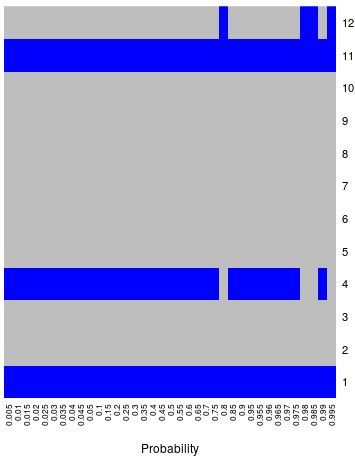
\includegraphics[width=0.4\linewidth]{Figuras/betas-mip/heatmap-exemplo-grupos}
%	\caption{}
%	\label{fig:heatmap-exemplo-grupos}
%\end{figure}
%
%
%\begin{eqnarray}
%\underset{\beta_{0\alpha},\beta_\alpha,z_{p \alpha}, \phi_{p \alpha}, \varepsilon_{t j}^{+},\varepsilon_{t j}^{-}}{\text{min}} & \sum_{j \in J} \sum_{t\in T}\left(\alpha\varepsilon_{t j}^{+}+(1-\alpha)\varepsilon_{tj}^{-}\right) \label{eq:mipgr0} \\
%\mbox{s.t } & \varepsilon_{t j}^{+}-\varepsilon_{t j}^{-}=y_{t}-\beta_{0 \alpha}-\sum_{p \in P}\beta_{p j}x_{t,p},& \qquad\forall t \in T ,\forall j \in J, \label{eq:mipgr1}\\
%& \varepsilon_{t j}^{+},\varepsilon_{t j}^{-}\geq0,&\qquad\forall t \in T ,\forall j \in J, \label{eq:mipgr2}\\
%& - M z_{p \alpha} \leq \beta_{p j} \leq M z_{p \alpha},&\qquad \forall j \in J, \forall p\in\{1,\dots,P\}, \label{eq:mipgr3}\\
%& \sum_{p \in P} z_{p \alpha} \leq K, & \qquad \forall j \in J, \label{eq:mipgr4}\\
%& z_{p \alpha} \in \{0,1\},&\qquad \forall j \in J, \forall p\in\{1,\dots,P\}, \label{eq:mipgr5}\\
%& \beta_{0\alpha} + \beta_{\alpha}^T x_{t} \leq \beta_{0\alpha'} + \beta_{\alpha'}^T x_{t}, & \qquad \forall t \in T, \forall (\alpha, \alpha') \in A \times A,  \alpha < \alpha',\nonumber\\ \label{eq:mipgr6} \\
%& z_{p\alpha} - z_{p\alpha+1} \leq m_{p\alpha}, & \qquad \forall j \in J', \qquad \forall p \in P  \\
%& \sum_{j \in J'} r_\alpha \leq |G| - 1 
%\label{eq:mipgr} \\
%\end{eqnarray}
%where $A' = A\setminus \{|A|\}$


\subsection{Variable selection via LASSO}
\label{sec:best-subset-ell1}

The second form of regularization we work here the LASSO technique. This method consists on the inclusion of the penalized coefficients $\ell_1$-norm on the objective function of the QR problem. In \cite{belloni_l1-penalized_2009}, the reader can find properties and convergence rates when using the LASSO to select variables in a quantile regression setting. 
The advantage of this method is that coefficients are shrunk towards zero by changing a continuous parameter $\lambda$, which penalizes the size of the $\ell_1$-norm.  
When the value of $\lambda$ gets bigger, fewer variables are selected to be used. 
This is the same strategy of the LASSO methodology, and its usage for the quantile regression is discussed in \cite{li2012l1}.
On the litterature, the LASSO QR regularization is applied for a single quantile only by the following optimization problem:
\begin{equation}
\underset{\beta_{0\alpha},\beta_\alpha}{\text{min}} \sum_{t \in T}\alpha|y_{t}-q_\alpha(x_t)|^{+}+ \sum_{t \in T}(1-\alpha)|y_{t}-q_\alpha(x_t)|^{-}+\lambda\|\beta_\alpha\|_{1},
\label{eq:l1-qar-optim}
\end{equation}
\[
q_\alpha(x_t)=\beta_{0}-\beta^T x_{t}.
\]
In our problem, however, we need to estimate multiple quantiles at once, in order to being able to circumvent the crossing quantiles issue. 

The process of estimation is done in two stages: (i) variable selection and (ii) coefficients estimation. At first, all normalized covariates\footnote{For such estimation to be coherent each covariate must have the same relative weight in comparison with one another, i.e., they must be normalized. 
This normalization process is a linear transformation to each covariate such that all have mean $\mu = 0$ and variance $\sigma^2 = 1$. 
We apply the transformation $\tilde{x}_{t,p} = (x_{t,p} - \bar{x}_{t,p}) / \hat\sigma_{x_{t,p}}$, where $\bar{x}_{t,p}$ and $\hat{\sigma}_{x_{t,p}}$ are respectively the sample's unconditional mean and standard deviation. The $\tilde{y}_{t-p,i}$ series will be used to estimate the coefficients, as this series has the desired properties.} are input on the following optimization problem:
\begin{IEEEeqnarray}{lr}
\tilde \beta_\lambda^{*} = \underset{\beta_{0j},\beta_j,\varepsilon_{t j}^{+},\varepsilon_{t j}^{-}}{\text{arg min}} \sum_{j \in J} \left( \sum_{t \in T}(\alpha_j\varepsilon_{t j}^{+}+(1-\alpha_j)\varepsilon_{t j}^{-}) \right. \span \nonumber \\
\span \left. +\lambda\sum_{p \in P} (\xi^+_{pj} + \xi^-_{pj}) \right)   \label{eq:obj-lasso} \\
\mbox{subject to } \nonumber & \\
\varepsilon_{t j}^{+}-\varepsilon_{t j}^{-}=y_{t}-\beta_{0 j}-\beta_{j}^T x_{t},& \forall t \in T ,\forall j \in J,\\
\xi^+_{pj} - \xi^-_{pj} = \beta_{p j},&\forall p\in P, \forall j \in J,  \label{l1-qar-3}
\\
\beta_{0j} + \beta_{j}^T x_{t} \leq \beta_{0,j+1} + \beta_{j+1}^T x_{t},&\forall t \in T, \forall j \in J_{(-1)}, \\
\varepsilon_{t j}^{+},\varepsilon_{t j}^{-}, \xi_{t j}^{+},\xi_{t j}^{-} \geq0,&\forall t \in T, \forall j \in J,\label{eq:obj-lasso-end}
\end{IEEEeqnarray}
This model is built upon the standard linear programming model for the quantile regression (\ref{eq:linear-opt-1})-(\ref{eq:linear-opt-ult}). 
On the above formulation, the $\ell_1$-norm of equation (\ref{eq:l1-qar-optim}) is substituted by the sum $\xi^+_{pj} + \xi^-_{pj}$, for each $j$, which represents the absolute value of $\beta_{pj}$. 

% % % % % % % % Esse trecho deve ser usado quando os coeficientes do lasso forem utilizados, e não apenas o lasso sendo um seletor de variáveis % % % % % % % % %
%Each component of the output $\tilde \beta_\lambda^{*LASSO}$ must be corrected by multiplying each coefficient for its standard deviation: $\beta_{p\alpha,\lambda}^{*LASSO} = \tilde \beta_{p\alpha,\lambda}^{*LASSO} \hat\sigma_{x_{t,p}}$.
%\begin{eqnarray}
%\tilde \beta_\lambda^{*LASSO} = \underset{\beta_{0},\beta,\varepsilon_{t j}^{+},\varepsilon_{t j}^{-}}{\text{arg min}} & \sum_{j \in J} \sum_{t \in T}\left(\alpha\varepsilon_{t j}^{+}+(1-\alpha)\varepsilon_{t j}^{-}\right)+\lambda\sum_{p \in P}\mbox{\ensuremath{\xi}}_{p \alpha} \label{eq:obj-lasso} \\
%\mbox{subject to } & \varepsilon_{t j}^{+}-\varepsilon_{t j}^{-}= y_{t}-\beta_{0 \alpha}-\sum_{p \in P}\beta_{p j}\tilde x_{t,p},&\forall t\in T, \forall j \in J, \\
%& \varepsilon_{t j}^{+},\varepsilon_{t j}^{-}\geq0,&\forall t \in T, \forall j \in J,\\
%& \xi_{pj}\geq\beta_{p j},&\forall p\in P, \forall j \in J,  \label{l1-qar-3}
%\\
%& \xi_{pj}\geq-\beta_{p j},&\forall p\in P, \forall j \in J.  \label{l1-qar-4}
%\end{eqnarray}

For low values of $\lambda$, the penalty over the size of coefficients is small, making the output of problem (\ref{eq:obj-lasso})-(\ref{eq:obj-lasso-end}) be composed mainly of nonzero coefficients. On the other hand, when the penalty on $\| \beta_j \|_1$ is big, many covariates will have zero valued coefficients. When $\lambda$ approaches infinity, one has a constant model. 
Note the linear coefficient $\beta_{0j}$ is not penalized.

As the LASSO coefficients are shrunk towards zero they become biased. Our strategy will be to employ the LASSO as a variable selector, and estimate coefficients with regular QR on a second stage. 
The optimum vector of coefficients $\tilde \beta_\lambda^{*}$ on the first stage may be composed by both nonzero and zero coefficients, for a given $\lambda$ . 
We then define $S_\lambda$ as the set of indexes of selected variables given by
\begin{equation*}
S_\lambda = \{ p \in \{ 1,\dots,P \} | \; |\tilde \beta^{*}_{\lambda,p}| \neq 0  \}.
\end{equation*}
Hence, we have that, for each $p \in \{ 1,\dots,P \}$,
$$\beta^{*LASSO}_{\lambda,p} = 0 \Longrightarrow \beta^{*}_{\lambda,p} = 0.$$

On the second stage, the optimal coefficient vector $\tilde \beta_\lambda^{*}$ is estimated by the non-regularized QR, where only variables that belongs to $S_\lambda$ are input:
\begin{IEEEeqnarray*}{lr} (\mathcal{L}_{\lambda}^{*},\beta_{\lambda}^{*})\overset{(obj,var)}{\longleftarrow} \underset{\beta_{0j},\beta_j,z_{p j}, \varepsilon_{t j}^{+},\varepsilon_{t j}^{-}}{\text{min}} \sum_{j \in J}  \sum_{t\in T}\left(\alpha_j \varepsilon_{t j}^{+}+(1-\alpha_j)\varepsilon_{tj}^{-}\right) \span \nonumber
\\
\text{subject to } \span \nonumber \\
\varepsilon_{t j}^{+}-\varepsilon_{t j}^{-}=y_{t} - \beta_{0\alpha} - \sum_{p\in S_\lambda} \beta_p x_{t,p}, & \forall t \in T, \forall j \in J, \\
\span \forall j \in J_{(-1)}, \forall p\in P, \\
\beta_{0j} + \beta_{j}^T x_{t} \leq \beta_{0,j+1} + \beta_{j+1}^T x_{t}, & \forall t \in T, \forall j \in J_{(-1)},\\
\varepsilon_{tj}^+,\varepsilon_{tj}^- \geq 0, &  \forall t \in T,\forall j \in J,\\ 
	 D2_{pj}^+, D2_{pj}^- \geq 0, & \forall j \in J,  \forall p\in P.
\end{IEEEeqnarray*}
The variable $\mathcal{L}_{\lambda}^{*}$ receives the value of the objective function on its optimal solution.
In summary, the optimization in equation \ref{eq:l1-qar-optim} acts as a variable selection for the subsequent estimation, which is normally called the post-LASSO estimation \cite{belloni2009least}.

\section{Regularization on the quantiles}

The nonparametric approach we use in this paper consists of a different model for each $\alpha$-quantile. From the assumption that the value of similar quantiles be produced by similar models, we need to prevent instabilities and big changes on the $p$ coefficient $\beta_p(\alpha)$ when seen as a function of probability $\alpha$. 
Another issue we find in practice is how the quantile estimation is less precise on the boundaries.

At first, we show an example to illustrate the aforementioned issues. We simulate 400 observations of the following AR(1) process:
\begin{equation}
	y_t = 0.6 y_{t-1} + \varepsilon_t, \quad \varepsilon_t \sim N(0, 1)
\end{equation} 
%To prevent initial value bias, we use 1000 observations as burn in and discard them.


Controlled experiment
- melhora a variancia
- as pontas são mais dificeis pra RQ
- no meio parece om ar1

In this controlled experiment, the results are shown on Figure \todoi{Colocar figura boxplot}. The main results are: (i) compared with the original QR model in \cite{koenker1978regression}, our estimator has statistically significant smaller variance (p-values shown on table \todoi{put table}); (ii) Extreme quantiles show larger variance than central quantiles; (iii) by using QR we can 


\begin{figure*}
	\centerline{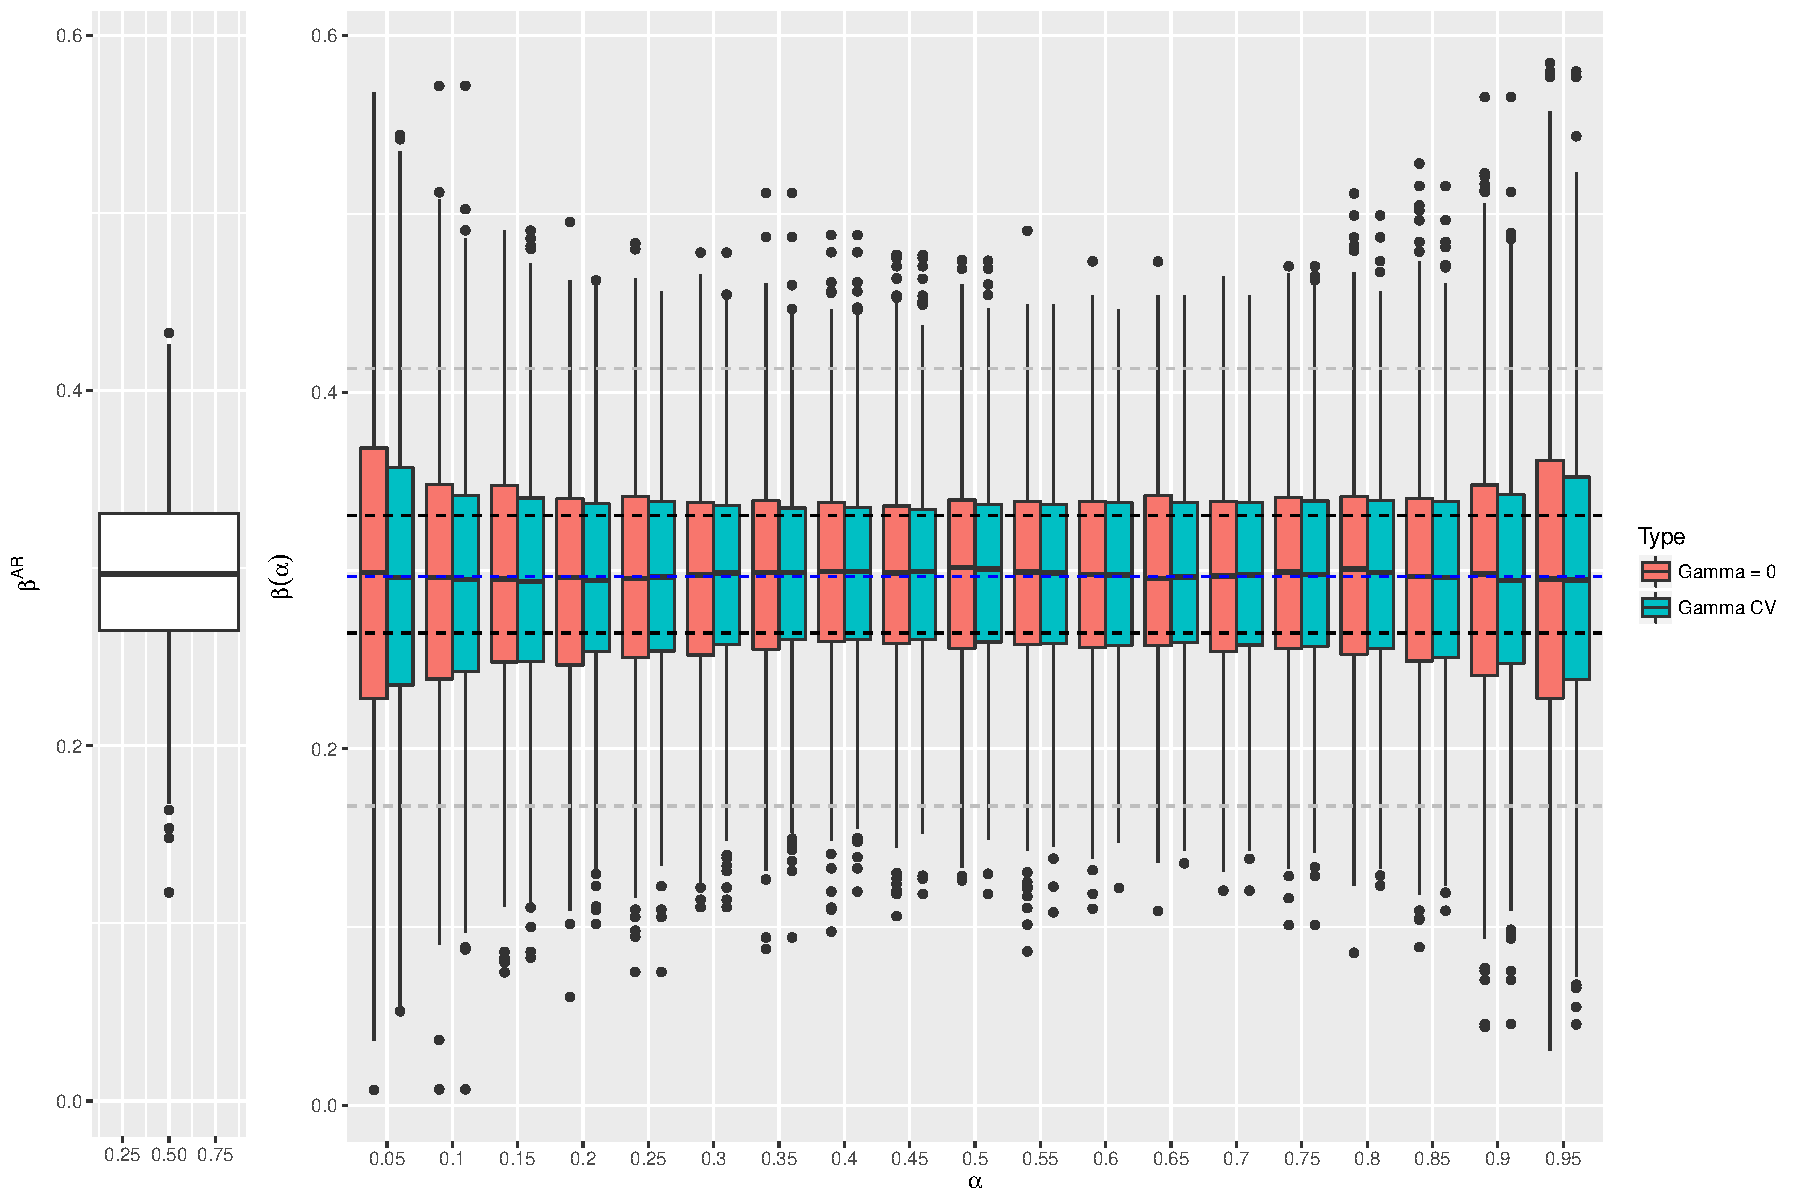
\includegraphics[width=7in]{Images/boxplot-ar1.pdf}}
\end{figure*}


% latex table generated in R 3.4.2 by xtable 1.8-2 package
% Thu Dec 14 13:21:18 2017
\begin{table}[ht]
\centering
\begin{tabular}{rr}
  \hline
Probability & P.values \\ 
  \hline
0.05 & 1.00 \\ 
  0.10 & 0.99 \\ 
  0.15 & 0.99 \\ 
  0.20 & 0.95 \\ 
  0.25 & 0.95 \\ 
  0.30 & 0.95 \\ 
  0.35 & 0.97 \\ 
  0.40 & 0.99 \\ 
  0.45 & 0.99 \\ 
  0.50 & 0.98 \\ 
  0.55 & 0.98 \\ 
  0.60 & 0.98 \\ 
  0.65 & 0.98 \\ 
  0.70 & 0.95 \\ 
  0.75 & 0.94 \\ 
  0.80 & 0.94 \\ 
  0.85 & 0.94 \\ 
  0.90 & 0.99 \\ 
  0.95 & 1.00 \\ 
   \hline
\end{tabular}
\end{table}



To see if this difference is significant, we use an $F$ test for the variance ratio. Let $X$ and $Y$ be two datasets from normally distributed random variables with $n$ and $m$ observations, respectively. The statistic $F = \frac{S^2_X}{S^2_Y}$ follows an $F$ distribution with $n-1$ and $m-1$ degrees of freedom.


\textit{iid} observations of random variable $y= 1 + \beta_1 $, where $X_1$ are normal explanatory variables. Let $X_{reg} = [X_1 \, X_2]$ be input on the problem and we have to figure out the real model.   shown on Figure \ref{fig:lasso-selection-normal}.
To force the model to have parsimony on the quantiles, we propose to penalize the second derivative of $\beta_p(\alpha)$. 
On the implementation side, we must limit the second difference of the sequence of coefficients $\{\beta_{pj}\}_{j \in J}$ for every parameter $p$. This will bring smoothness to $\beta_p(\alpha)$.
\begin{figure}
	\centering
	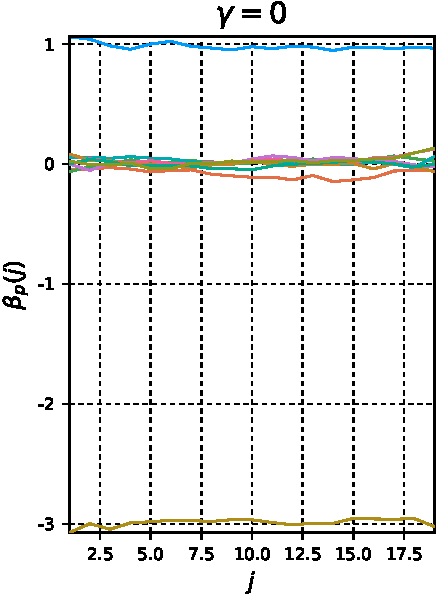
\includegraphics[width=0.5\linewidth]{Images/Lambda10-gamma03-cropped}
	\caption{$\mathcal{K}$-fold CV and $\mathcal{K}$-fold with non-dependent data. Observations in blue are used to estimation and in orange for evaluation. Note that non-dependent data doesn't use all dataset in each fold.}
	\label{fig:lasso-selection-normal}
\end{figure}

\begin{equation}
\tilde{D}_{pj}^{2}:=\frac{\left(\frac{\beta_{p,j+1}-\beta_{pj}}{\alpha_{j+1}-\alpha_{j}}\right)-\left(\frac{\beta_{p,j}-\beta_{p,j-1}}{\alpha_{j}-\alpha_{j-1}}\right)}{\alpha_{j+1}-2\alpha_{j}+\alpha_{j-1}}.
\end{equation}
This idea is implemented on the optimization problem by adding a penalty on the objective function to penalize the absolute value $|D_{pj'}^{2}|$ by a tuning parameter $\gamma$, that controls how rough the sequence $\{\beta_{pj}\}_{j \in J}$ can be. The full optimization problem for the best subset selection via MILP which incorporates the derivative penalty is given below:
\begin{IEEEeqnarray}{lr}
	\underset{\beta_{0j},\beta_j,z_{p j} \varepsilon_{t j}^{+},\varepsilon_{t j}^{-}}{\text{min}} \sum_{j \in J} \sum_{t\in T}\left(\alpha_j\varepsilon_{t j}^{+}+(1-\alpha_j)\varepsilon_{tj}^{-}\right) \nonumber \span \\
	\span + \gamma \sum_{j \in J'} (D2_{pj}^+ + D2_{pj}^-)   \\
	\mbox{subject to} \span \nonumber \\
	\varepsilon_{t j}^{+}-\varepsilon_{t j}^{-}=y_{t}-\beta_{0 j}-\beta_{j}^T x_{t,p},& \forall t \in T ,\forall j \in J,\\
	- M z_{p \alpha} \leq \beta_{p j} \leq M z_{p \alpha}, & \forall j \in J, \forall p\in P, \\
	\sum_{p \in P} z_{p \alpha} \leq K, & \forall j \in J, \\
	D2_{pj}^+ - D2_{pj}^- = \frac{\left(\frac{\beta_{p,j+1}-\beta_{pj}}{\alpha_{j+1}-\alpha_{j}}\right)-\left(\frac{\beta_{p,j}-\beta_{p,j-1}}{\alpha_{j}-\alpha_{j-1}}\right)}{\alpha_{j+1}-2\alpha_{j}+\alpha_{j-1}}, \span   \nonumber \\
	\span \forall j \in J_{(-1)}, \forall p\in P, \\
	\beta_{0j} + \beta_{j}^T x_{t} \leq \beta_{0,j+1} + \beta_{j+1}^T x_{t},&\forall t \in T, \forall j \in J_{(-1)}, \\
	z_{p \alpha} \in \{0,1\}, & \forall j \in J,  \forall p\in P, \\
	\varepsilon_{t j}^{+},\varepsilon_{t j}^{-}\geq0, & \forall t \in T ,\forall j \in J, \\
	D2_{pj}^+, D2_{pj}^- \geq 0, & \forall j \in J,  \forall p\in P.
\end{IEEEeqnarray}
where $A'$ is the set formed by the same elements of $A$ without the first and the last elements, that need to be taken out of the sum as their second derivative cannot be calculated.
The sum $D2_{pj}^+ + D2_{pj}^-$ represents the absolute value of the second derivative, and its penalty is tuned by parameter $\gamma$.

The same feature is incorporated in the LASSO estimation, which now incorporates penalization  of both coefficients $\ell_1$-norm as well as the second derivative of $\beta(\alpha)$, shown by the problem below: 
The modified LASSO problem to include the 

\begin{IEEEeqnarray}{lr}
	\tilde \beta_\lambda^{*LASSO} = \underset{\beta_{0},\beta,\varepsilon_{t j}^{+},\varepsilon_{t j}^{-}}{\text{arg min}} \sum_{j \in J} \sum_{t \in T}(\alpha_j\varepsilon_{t j}^{+}+(1-\alpha_j)\varepsilon_{t j}^{-}) \span \nonumber \\
	\span + \lambda \sum_{p \in P} (\xi^+_{pj} + \xi^-_{pj}) + \gamma \sum_{j \in J'} (D2_{pj}^+ + D2_{pj}^-)  \label{eq:obj-lasso-2reg} \\
	\mbox{subject to } \nonumber & \\
	\varepsilon_{t j}^{+}-\varepsilon_{t j}^{-}=y_{t}-\beta_{0 j}-\beta_{j}^T x_{t,p},& \forall t \in T ,\forall j \in J,\\
	\xi_{pj}\geq\beta_{p j},&\forall p\in P, \forall j \in J, 
	\\
	\xi_{pj}\geq - \beta_{p j},&\forall p\in P, \forall j \in J,  
	\\
	D2_{pj}^+ - D2_{pj}^- = \frac{\left(\frac{\beta_{p,j+1}-\beta_{pj}}{\alpha_{j+1}-\alpha_{j}}\right)-\left(\frac{\beta_{p,j}-\beta_{p,j-1}}{\alpha_{j}-\alpha_{j-1}}\right)}{\alpha_{j+1}-2\alpha_{j}+\alpha_{j-1}}, \span   \nonumber \\
	\span \forall j \in J_{(-1)}, \forall p\in P, \\
	\beta_{0j} + \beta_{j}^T x_{t} \leq \beta_{0,j+1} + \beta_{j+1}^T x_{t},&\forall t \in T, \forall j \in J_{(-1)}, \\
	\varepsilon_{t j}^{+},\varepsilon_{t j}^{-}\geq0,&\forall t \in T, \forall j \in J,\\
	D2_{pj}^+, D2_{pj}^- \geq 0, & \forall j \in J,  \forall p\in P. \label{eq:obj-lasso-2reg-end} 
\end{IEEEeqnarray}

\subsection{ADALASSO}
A popular extension of the LASSO is the Adaptive LASSO (ADALASSO). In \cite{ciuperca_adaptive_2016}, the authors extended the ADALASSO for QR and have shown properties of the ADALASSO for the QR .

When estimating the ADALASSO for quantile regression, we show a few adaptations and extensions of the original method. The full process consists of two steps, each consisting of a LASSO estimation:
\begin{itemize}
	\item \textbf{First step:} First LASSO regularization, as in problem (\ref{eq:obj-lasso-2reg})-(\ref{eq:obj-lasso-2reg-end}).
	
	\item \textbf{Second step:} The coefficients of the LASSO estimation are used to form the weights $w_{pj}$  are:
	\begin{enumerate}
		\item $w_{pj} = 1/ \beta_{pj}$.
		\item $w_{pj} = 1/ (\beta_{pj} \parallel \beta_j \parallel_1)$,
	\end{enumerate}
	where $\beta_{pj}$ stands for the coefficients obtained on the first step and $\parallel \beta_j \parallel_1$ is the $\ell_1$-norm of the $j$\textsuperscript{th} quantile coefficients.
	The weights $w_j$ are input to a second-stage Lasso estimation:
	\begin{IEEEeqnarray*}{lr}
		\underset{\beta_{0j},\beta_j}{\text{min}} \sum_{j \in J} \left( \sum_{t\in T}\rho_{\alpha_j}(y_{t}-(\beta_{0j} + \beta_j^T x_t)) + \lambda\  \sum_{p \in P} w_{pj}^\delta \mid  \beta_{pj} \mid \right) \span \\
		\span + \gamma \sum_{j \in J'} (D2_{pj}^+ + D2_{pj}^-),
	\end{IEEEeqnarray*}
	where $\delta$ is an exponential parameter, normally set to 1.
\end{itemize}

%
%
%\begin{IEEEeqnarray*}{lr} (\mathcal{L}_{\lambda}^{*},\beta_{\lambda}^{*})\overset{(obj,var)}{\longleftarrow} \underset{\beta_{0j},\beta_j,z_{p j}, \varepsilon_{t j}^{+},\varepsilon_{t j}^{-}}{\text{min}} \sum_{j \in J} \sum_{t\in T}\left(\alpha_j \varepsilon_{t j}^{+}+(1-\alpha_j)\varepsilon_{t\alpha_j}^{-}\right) \span \nonumber
%	\\
%	&  + \gamma \sum_{j \in J'} (D2_{pj}^+ + D2_{pj}^-) \\
%	\text{subject to } \span \nonumber \\
%	\varepsilon_{t j}^{+}-\varepsilon_{t j}^{-}=y_{t} - \beta_{0\alpha} - \sum_{p\in S_\lambda} \beta_p x_{t,p}, & \forall t \in T, \forall j \in J, \\
%	D2_{pj}^+ - D2_{pj}^- = \frac{\left(\frac{\beta_{p,j+1}-\beta_{pj}}{\alpha_{j+1}-\alpha_{j}}\right)-\left(\frac{\beta_{p,j}-\beta_{p,j-1}}{\alpha_{j}-\alpha_{j-1}}\right)}{\alpha_{j+1}-2\alpha_{j}+\alpha_{j-1}}, \span   \nonumber \\
%	\span \forall j \in J_{(-1)}, \forall p\in P, \\
%	\beta_{0j} + \beta_{j}^T x_{t} \leq \beta_{0,j+1} + \beta_{j+1}^T x_{t}, & \forall t \in T, \forall j \in J_{(-1)},\\
%	\varepsilon_{tj}^+,\varepsilon_{tj}^- \geq 0, &  \forall t \in T,\forall j \in J,\\ 
%	D2_{pj}^+, D2_{pj}^- \geq 0, & \forall j \in J,  \forall p\in P.
%\end{IEEEeqnarray*}